\section{گام دوم: ساخت هرم لاپلاسی ۸ مرحله‌ای (بخش ۱)}

در این مرحله، هدف ما ساخت یک هرم لاپلاسی \lr{(Laplacian Pyramid)} با ۸ سطح برای هر یک از تصاویر است. هرم لاپلاسی ابزار بسیار قدرتمندی برای جداسازی باندهای فرکانسی تصویر است. لایه‌های پایین‌تر (تصاویر بزرگتر) فرکانس‌های بالا مانند لبه‌ها و جزئیات ظریف را در خود جای داده‌اند و هرچه به سمت لایه‌های بالاتر (تصاویر کوچکتر) می‌رویم، فرکانس‌های پایین‌تر و ساختار کلی تصویر باقی می‌ماند.

\begin{stepbox}
\field{روند ساخت هرم لاپلاسی}{
ابتدا باید یک هرم گوسی \lr{(Gaussian Pyramid)} بسازیم؛ به این شکل که تصویر را در هر مرحله تار کرده و ابعاد آن را نصف می‌کنیم. سپس برای استخراج جزئیات (هرم لاپلاسی)، هر لایه از هرم گوسی را بزرگ کرده و از لایه‌ی قبلی‌اش کم می‌کنیم.
}
\end{stepbox}

\subsection{پیاده‌سازی کد}

کد این بخش را برای درک بهتر به دو قسمت تقسیم کرده‌ایم. در تابع اول، هرم گوسی را ساخته و سپس از روی آن هرم لاپلاسی را استخراج می‌کنیم:

\begin{codebox}[\lr{Generate Laplacian Pyramid}]
\begin{lstlisting}[language=Python]
def generate_laplacian_pyramid(img, levels=8):
    gaussian_pyramid = [img]
    current_img = img
    
    for i in range(levels - 1):
        current_img = cv2.pyrDown(current_img)
        gaussian_pyramid.append(current_img)
\end{lstlisting}
\end{codebox}

در خطوط بالا، لیست \lr{\texttt{gaussian\_pyramid}} با تصویر اصلی مقداردهی اولیه می‌شود. سپس در یک حلقه، تابع \lr{\texttt{cv2.pyrDown}} تصویر را تار کرده و ابعاد آن را نصف می‌کند و به لیست اضافه می‌نماید تا ۸ سطح تکمیل شود.

حالا به سراغ استخراج جزئیات می‌رویم:

\begin{warnbox}[خطای اختلاف ابعاد در \lr{OpenCV}]
هنگام استفاده از \lr{\texttt{cv2.pyrUp}} برای بزرگنمایی تصویر، اگر ابعاد تصویر اولیه فرد باشد، یک پیکسل در بازسازی اختلاف ایجاد می‌شود. برای جلوگیری از این ارور، از تکنیک برش \lr{(Slicing)} ماتریس برای هم‌سایز کردن دقیق لایه‌ها استفاده کرده‌ایم.
\end{warnbox}

\begin{codebox}[\lr{Calculate Laplacian Layers}]
\begin{lstlisting}[language=Python]
    laplacian_pyramid = []
    
    for i in range(levels - 1):
        gaussian_current = gaussian_pyramid[i]
        gaussian_next = gaussian_pyramid[i + 1]
        
        gaussian_expanded = cv2.pyrUp(gaussian_next)
        
        h, w = gaussian_current.shape
        gaussian_expanded = gaussian_expanded[:h, :w]
        
        laplacian = cv2.subtract(gaussian_current, gaussian_expanded)
        laplacian_pyramid.append(laplacian)
        
    laplacian_pyramid.append(gaussian_pyramid[-1])
    
    return laplacian_pyramid
\end{lstlisting}
\end{codebox}

در این بخش، لایه‌ی کوچکتر (\lr{\texttt{gaussian\_next}}) را با \lr{\texttt{pyrUp}} بزرگ می‌کنیم. متغیرهای \lr{\texttt{h}} و \lr{\texttt{w}} ابعاد لایه‌ی فعلی را می‌گیرند تا تصویر بزرگ‌شده دقیقاً با آن هم‌اندازه برش بخورد. در نهایت با \lr{\texttt{cv2.subtract}} اختلاف این دو را محاسبه می‌کنیم که همان فرکانس‌های بالای تصویر است.

برای نمایش این لایه‌ها کنار هم، نیاز به یک بوم خالی داریم:

\begin{codebox}[\lr{Build Composite Image}]
\begin{lstlisting}[language=Python]
def build_composite_pyramid(pyramid):
    total_width = sum([img.shape[1] for img in pyramid])
    max_height = pyramid[0].shape[0]
    
    composite = np.zeros((max_height, total_width), dtype=np.float32)
    
    current_x = 0
    for img in pyramid:
        h, w = img.shape
        normalized_img = cv2.normalize(img, None, 0, 255, cv2.NORM_MINMAX)
        
        composite[0:h, current_x:current_x + w] = normalized_img
        current_x += w
        
    return composite
\end{lstlisting}
\end{codebox}

در تابع بالا، ابتدا مجموع عرض تمام لایه‌ها برای تعیین \lr{\texttt{total\_width}} محاسبه شده و یک ماتریس صفر \lr{(Canvas)} ساخته می‌شود. 
از آنجایی که تفریق ماتریس‌ها در هرم لاپلاسی اعداد منفی تولید می‌کند، حتماً باید از تابع \lr{\texttt{cv2.normalize}} استفاده کنیم تا مقادیر به بازه‌ی استاندارد نمایش (۰ تا ۲۵۵) نگاشت شوند. متغیر \lr{\texttt{current\_x}} نیز مشخص می‌کند تصویر بعدی دقیقاً از کجای محور افقی چسبانده شود.

\subsection{خروجی هرم‌های لاپلاسی}

پس از اعمال توابع فوق بر روی هر چهار تصویر، خروجی‌های یکپارچه‌ی زیر حاصل می‌شود که به خوبی توزیع فرکانس‌ها را از چپ (جزئیات) به راست (کلیات) نشان می‌دهند:

\begin{figure}[h!]
    \centering
    \begin{subfigure}{0.48\textwidth}
        \centering
        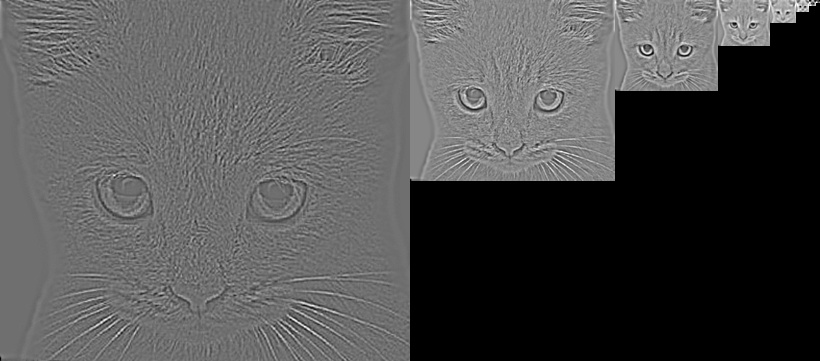
\includegraphics[width=\textwidth]{images/Laplacian_Near_Set1.jpg}
        \caption{هرم تصویر \lr{Near} (گربه)}
    \end{subfigure}
    \hfill
    \begin{subfigure}{0.48\textwidth}
        \centering
        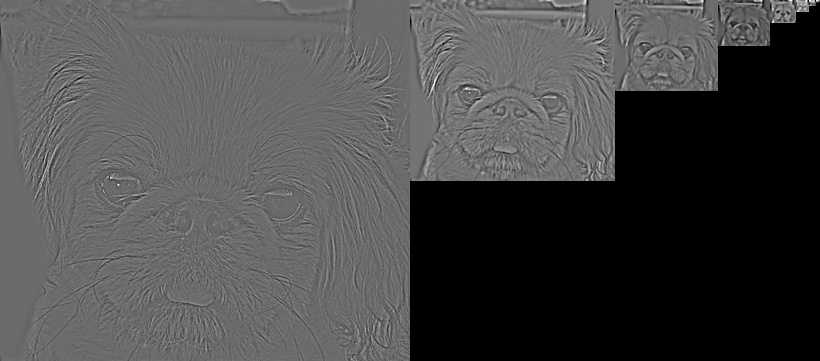
\includegraphics[width=\textwidth]{images/Laplacian_Far_Set1.jpg}
        \caption{هرم تصویر \lr{Far} (سگ)}
    \end{subfigure}
    
    \vspace{0.5cm}
    
    \begin{subfigure}{0.48\textwidth}
        \centering
        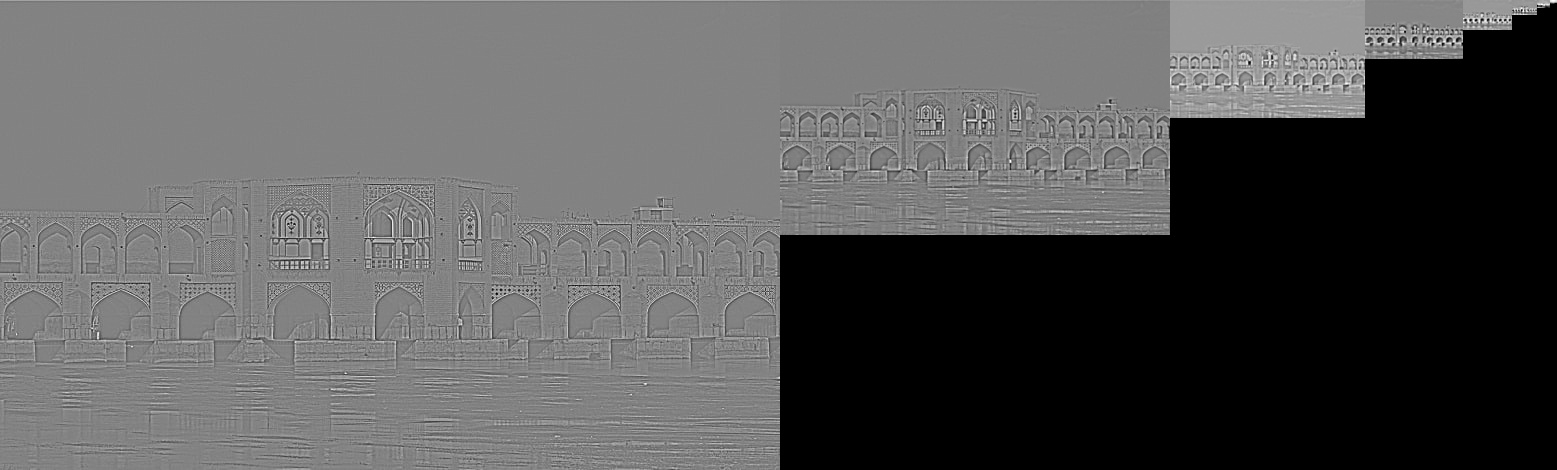
\includegraphics[width=\textwidth]{images/Laplacian_Near_Set2.jpg}
        \caption{هرم تصویر \lr{Near} (پل)}
    \end{subfigure}
    \hfill
    \begin{subfigure}{0.48\textwidth}
        \centering
        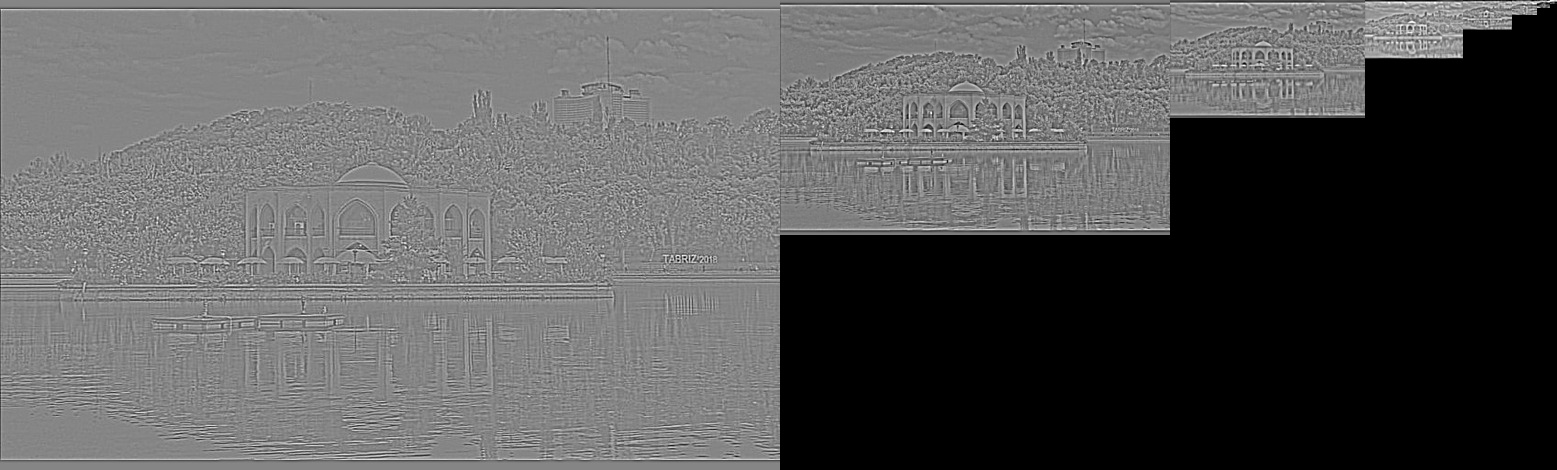
\includegraphics[width=\textwidth]{images/Laplacian_Far_Set2.jpg}
        \caption{هرم تصویر \lr{Far} (منظره)}
    \end{subfigure}
    \caption{تصاویر یکپارچه هرم لاپلاسی برای مجموعه‌های اول و دوم}
    \label{fig:laplacian_pyramids}
\end{figure}